% Credits to Jan Küster for providing a nice CV template:
% https://github.com/jankapunkt/latexcv/tree/master/sidebarleft

% RequirePackage can be used before documentclass, whille usepackage cannot.
% T1 is an 8-bit font encoding, while the TeX default is the 7-bit OT1
\RequirePackage[T1]{fontenc}
\documentclass[10pt]{article}

% we use utf8 since we want to build from any machine
\usepackage[utf8]{inputenc}

% provides \isempty test
\usepackage{xstring, xifthen}

% tex-live font
\usepackage[default]{raleway}

% select Adobe Times Roman as default font
%\usepackage{times}

% set up the use of sans font as a default
\renewcommand{\familydefault}{\sfdefault}

% more font size definitions
\usepackage{moresize}

% include fontawesome icon set
\usepackage{fontawesome}

% use to vertically center content
% [1] is the number of parameters the new command will take
% any settings set within this group will be confined to this group only
\newcommand{\vcenteredinclude}[1]{\begingroup
  % create horizontal box and assign it to box register 0
  % box registers are temporary storage spaces used for holding content that can be later inserted into the doc
  % box registers are numbered from 0 to 255
  % here the box register will contain the graphics given as parameter
  % after creating a box, u can use later in your document by using \box0
  \setbox0=\hbox{\includegraphics{#1}}
  % create a parbox, which is a box that can contain text and other elements
  % the term parbox is a combination of paragraph and box
  % parbox is particularly useful when u want to create a mini-page or a box with specific width and height,
  % and u want the text inside to be formatted like a paragraph
  % parbox has 2 required args: width and content
  % \wd0 will give you the width of box register 0  
  \parbox{\wd0}{\box0}
\endgroup}

% use to vertically center content
% the * after newcommand forbids paragraph tokens, be it those generated
% by blank lines or those generated by \par 
\newcommand*{\vcenteredhbox}[1]{\begingroup
  \setbox0=\hbox{#1}\parbox{\wd0}{\box0}
\endgroup}

% icon shortcut
\newcommand{\icon}[2] { 	
  % makebox command for the picture environment
  % u must specify a widht and a height in multiples of \unitlength
  % makebox creates a box just wide enough to contain the text specified
  \makebox(#2, #2){\textcolor{maincol}{
  % with csname, u can go from a list of character tokens to a control sequence
  \csname fa#1\endcsname
  }}
}

% icon with text shortcut
\newcommand{\icontext}[4]{
  % \mpwidth will be defined later
  \vcenteredhbox{\icon{#1}{#2}}  \hspace{2pt}  \parbox{0.9\mpwidth}{
  % 2 params: color and text
  \textcolor{#4}{#3}
  }
}

% icon with website url
\newcommand{\iconhref}[5]{ 						
    \vcenteredhbox{\icon{#1}{#2}}  \hspace{2pt} \small\href{#4}{\textcolor{#5}{#3}}
}

% icon with email link
\newcommand{\iconemail}[5]{ 						
    \vcenteredhbox{\icon{#1}{#2}}  \hspace{0pt} \href{mailto:#4}{
      \textcolor{#5}{#3}
    }
}

%-----------------------------------------------
%	PAGE LAYOUT  DEFINITIONS
%-----------------------------------------------

% page outer frames (debug-only)
% \usepackage{showframe}

% use paracol to display breakable two columns
\usepackage{paracol}

% define page styles using geometry
\usepackage[a4paper]{geometry}

% remove all possible margins
\geometry{top=1cm, bottom=1cm, left=1cm, right=1cm}

% fancyhydr provides facilities for constructing headers & footers,
% and for controlling their use
\usepackage{fancyhdr}
% produce empty heads and feet. No page numbers nor headings
\pagestyle{empty}

% space between header and content
% \setlength{\headheight}{0pt}

% paragraph indentation to zero
\setlength{\parindent}{0mm}

%-----------------------------------------------
%	TABLE /ARRAY DEFINITIONS
%-----------------------------------------------

% extended aligning of tabular cells
\usepackage{array}

% custom column right-align with fixed width
% use like p{size} but via x{size}
\newcolumntype{x}[1]{%
  >{\raggedleft\hspace{0pt}}p{#1}
}%

%-----------------------------------------------
%	GRAPHICS DEFINITIONS
%-----------------------------------------------

%for header image
\usepackage{graphicx}

% use this for floating figures
% \usepackage{wrapfig}
% \usepackage{float}
% \floatstyle{boxed} 
% \restylefloat{figure}

%for drawing graphics		
\usepackage{tikz}				
\usetikzlibrary{shapes, backgrounds,mindmap, trees}

%-----------------------------------------------
%	COLOR DEFINITIONS
%-----------------------------------------------

% defines \transparent and \texttransparent
% they are used like \color and \textcolot,
% except that the first arg is the transparency
\usepackage{transparent}
\usepackage{color}

% primary color
%\definecolor{maincol}{RGB}{ 225, 0, 0 } % red
%\definecolor{maincol}{RGB}{ 46, 139, 87 } % seagreen
\definecolor{maincol}{RGB}{ 0, 128, 128 } % teal
%\definecolor{maincol}{RGB}{ 70, 130, 180 } % steelblue

% accent color, secondary
% \definecolor{accentcol}{RGB}{ 250, 150, 10 }

% dark color
\definecolor{darkcol}{RGB}{ 70, 70, 70 }

% light color
\definecolor{lightcol}{RGB}{245,245,245}


% Package for links, must be the last package used
\usepackage[hidelinks]{hyperref}

% returns minipage width minus two times \fboxsep
% to keep padding included in width calculations.
% Can also be used for other boxes / environments
\newcommand{\mpwidth}{\linewidth-\fboxsep-\fboxsep}



%===============================================%
%
%	CV COMMANDS
%
%===============================================%

%-----------------------------------------------
%	 CV LIST
%-----------------------------------------------

% renders a standard latex list but abstracts away the environment definition (begin/end)
\newcommand{\cvlist}[1] {
	\begin{itemize}{#1}\end{itemize}
}

%-----------------------------------------------
%	 CV TEXT
%-----------------------------------------------

% base class to wrap any text based stuff here. Renders like a paragraph.
% Allows complex commands to be passed, too.
% param 1: *any
\newcommand{\cvtext}[1] {
	\begin{tabular*}{1\mpwidth}{p{0.98\mpwidth}}
		\parbox{1\mpwidth}{#1}
	\end{tabular*}
}

%-----------------------------------------------
%	 CV SECTION
%-----------------------------------------------

% Renders a a CV section headline with a nice underline in main color.
% param 1: section title
\newcommand{\cvsection}[1] {
	\vspace{14pt}
	\cvtext{
		\textbf{\LARGE{\textcolor{darkcol}{\uppercase{#1}}}}\\[-4pt]
		\textcolor{maincol}{ \rule{0.1\textwidth}{2pt} } \\
	}
}

%-----------------------------------------------
%	 META SKILL
%-----------------------------------------------

% Renders a progress-bar to indicate a certain skill in percent.
% param 1: name of the skill / tech / etc.
% param 2: level (for example in years)
% param 3: percent, values range from 0 to 1
\newcommand{\cvskill}[3] {
	\begin{tabular*}{1\mpwidth}{p{0.82\mpwidth}  r}
    \textcolor{black}{\textbf{#1}} & \textcolor{maincol}{#2}\\
	\end{tabular*}%

	\hspace{4pt}
	\begin{tikzpicture}[scale=1,rounded corners=2pt,very thin]
		\fill [lightcol] (0,0) rectangle (1\mpwidth, 0.15);
		\fill [maincol] (0,0) rectangle (#3\mpwidth, 0.15);
  \end{tikzpicture}%
}

%-----------------------------------------------
%	 CV EVENT
%-----------------------------------------------

% Renders a table and a paragraph (cvtext) wrapped in a parbox (to ensure minimum content
% is glued together when a pagebreak appears).
% Additional Information can be passed in text or list form (or other environments).
% the work you did
% param 1: time-frame i.e. Sep 14 - Jan 15 etc.
% param 2:	 event name (job position etc.)
% param 3: Customer, Employer, Industry
% param 4: Short description
% param 5: work done (optional)
% param 6: technologies include (optional)
% param 7: achievements (optional)
\newcommand{\cvevent}[7] {
	% we wrap this part in a parbox, so title and description are not separated on a pagebreak
	% if you need more control on page breaks, remove the parbox
	\parbox{\mpwidth}{
		\begin{tabular*}{1\mpwidth}{p{0.72\mpwidth}  r}
			\textcolor{black}{\textbf{#2}} & \colorbox{maincol}{
				\makebox[0.27\mpwidth]{\textcolor{white}{#1}}
			} \\
			\textcolor{maincol}{\textbf{#3}} & \\
		\end{tabular*}\\[8pt]

		\ifthenelse{\isempty{#4}}{}{
			\cvtext{#4}\\
		}
	}

	\ifthenelse{\isempty{#5}}{}{
		\vspace{9pt}
		{#5}
	}

	\ifthenelse{\isempty{#6}}{}{
		\vspace{9pt}
		\cvtext{\textbf{Technologies include:}}\\
		{#6}
	}

	\ifthenelse{\isempty{#7}}{}{
		\vspace{9pt}
		\cvtext{\textbf{Achievements include:}}\\
		{#7}
	}
	\vspace{14pt}
}

%-----------------------------------------------
%	 CV META EVENT
%-----------------------------------------------

% Renders a CV event on the sidebar
% param 1: title
% param 2: subtitle (optional)
% param 3: customer, employer, etc,. (optional)
% param 4: info text (optional)
\newcommand{\cvmetaevent}[4] {
	\textcolor{maincol} {\cvtext{\textbf{\begin{flushleft}#1\end{flushleft}}}}

	\ifthenelse{\isempty{#2}}{}{
	\textcolor{darkcol} {\cvtext{\textbf{#2}} }
	}

	\ifthenelse{\isempty{#3}}{}{
		\cvtext{{ \textcolor{darkcol} {#3} }}\\
	}

	\cvtext{#4}\\[14pt]
}

%-----------------------------------------------
%	 QR CODE
%-----------------------------------------------

% Renders a qrcode image (centered, relative to the parentwidth)
% param 1: percent width, from 0 to 1
\newcommand{\cvqrcode}[1] {
	\begin{center}
		
\includegraphics[width={#1}\mpwidth]{qrcode}
	\end{center}
}


%===============================================%
%
%	DOCUMENT CONTENT
%
%===============================================%
\begin{document}
\columnratio{0.31}
\setlength{\columnsep}{2.2em}
\setlength{\columnseprule}{4pt}
\colseprulecolor{lightcol}

\begin{paracol}{2}
\begin{leftcolumn}
 %-----------------------------------------------
 %	 CV IMAGE
 %-----------------------------------------------
 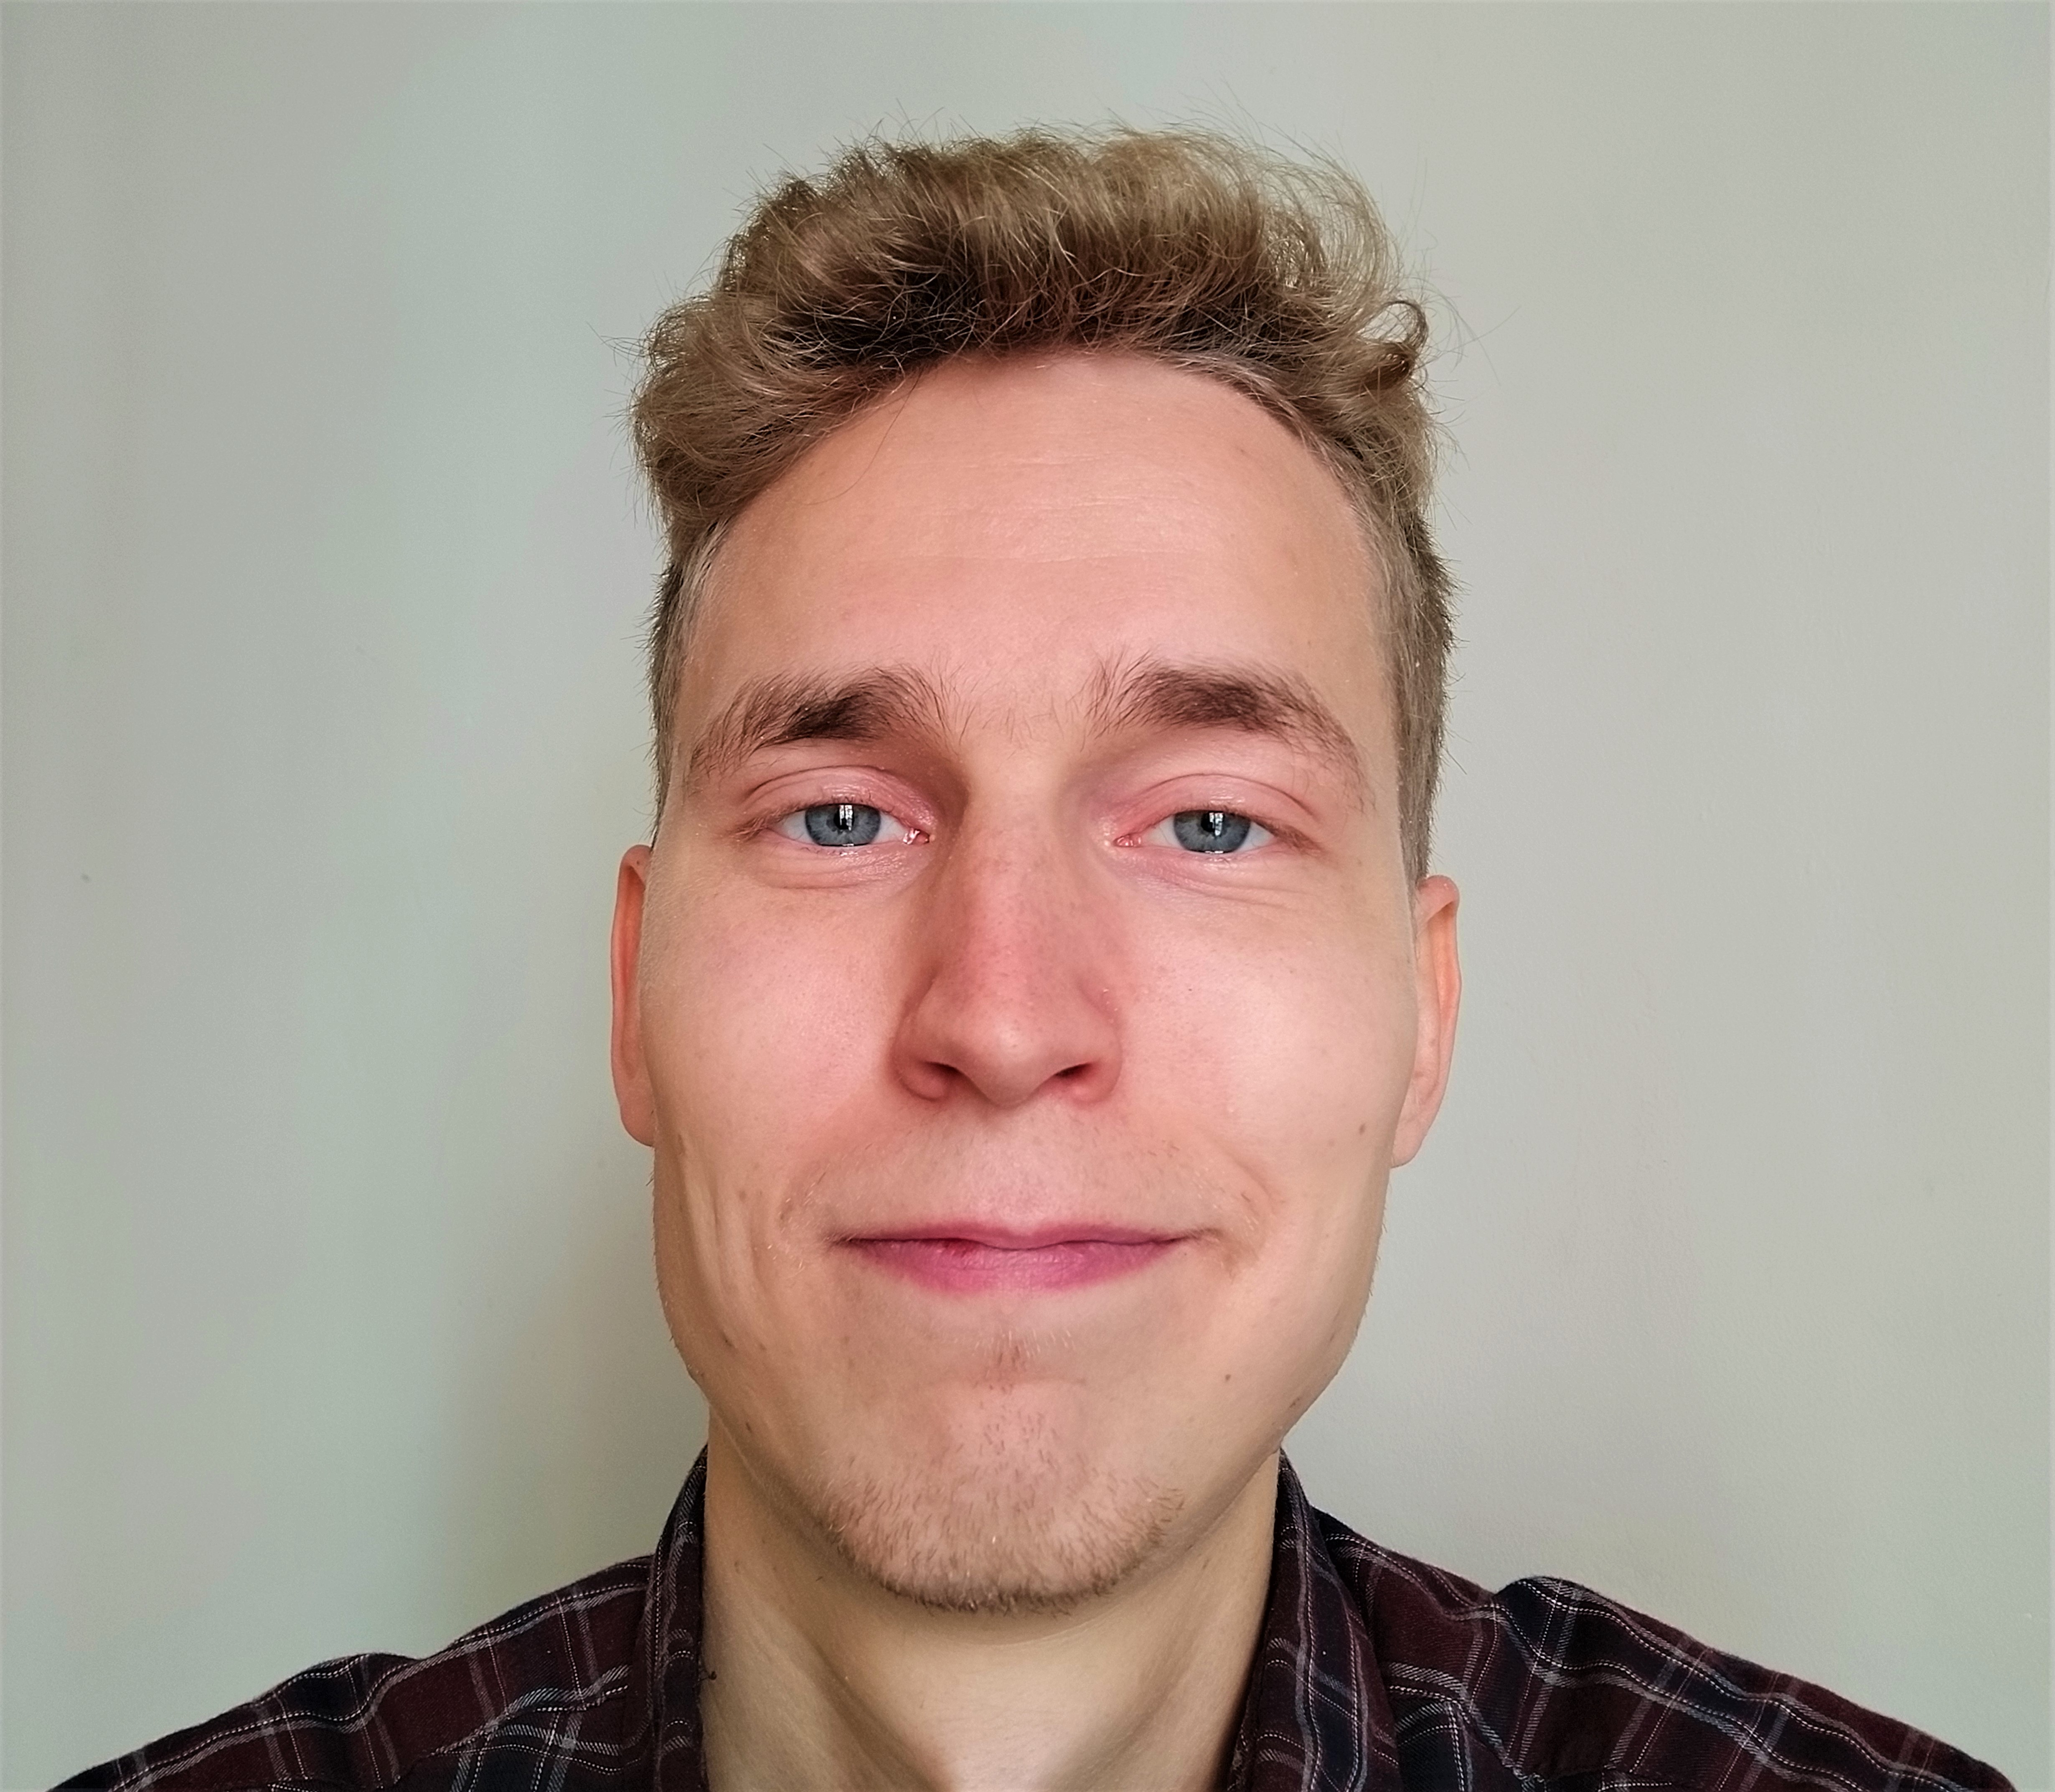
\includegraphics[width=\linewidth]{CV_kuva.jpg}

 %-----------------------------------------------------------------------------
 %       NAME
 %-----------------------------------------------------------------------------

 \vspace{2mm}
 \colorbox{darkcol}{
 % minipage has 3 optional args:
 % [position][height][inner-pos]
 % position determines the vertical alignment relative to the text line.
 % by default, the alignment is center.
 % height specifies the height of the minipage
 % inner-pos controls the vertical placement of the contents inside the box
 % takes 1 mandatory arg: text-width
 \begin{minipage}[c][1cm][c]{.97\mpwidth}
  \begin{center}
   \LARGE{
	\textbf{
	 \textcolor{white}{Akseli Ingervo}
	}
   }
  \end{center}
 \end{minipage}
 }

 %-----------------------------------------------
 %	 PROFILE
 %-----------------------------------------------

 % add some space between picture and profile
 % vfill is a TeX primitive
 % it produces a rubber length whcih can stretch or shrink vertically
 % rubber lengths have a natural length + a degree of elasticity
 % e.g., the \fill length command has a natural len of 0 but is infinitely
 % stretchable
 % \vfill ends the paragraph at the spot and adds the filling vertical space
 %\vfill

 % \null is the same as \hbox{}
 % is tan be used for a material which reserves no space but shows TeX that
 % there is a box which is taken into account for typesetting
 %\null
 \cvsection{PROFILE}

 \small\cvtext{
  I am a Master of Political Science, who is engaging on a new career path. After working a few years in the banking sector, I decided to follow my passion began studying computer science. Through my own projects and my studies, I've acquired experience about full stack development, data science, and algorithms. I am now seeking a summer job that would enable me to step up my knowledge about cloud engineering.
 } \\[4mm]

 %-----------------------------------------------
 %	 SKILLS
 %-----------------------------------------------
 \vfill
 %\hskip 0pt plus 1filll
 \cvsection{SKILLS}

 \cvskill{Python}{> 2 v}{1}

 \cvskill{JavaScript}{2 v}{0.8}

 \cvskill{HTML ja CSS}{2 v}{0.75}

 \cvskill{Linux}{> 2 v}{0.7}

 \cvskill{SQL}{1 v}{0.5}

 \cvskill{Node.js}{1 v}{0.5}

 \cvskill{Express}{< 1 v}{0.4}

 \cvskill{Git}{1 v}{0.4}

 \cvskill{Django}{< 1 v}{0.2}


 %-----------------------------------------------
 %	 CONTACT
 %-----------------------------------------------
 \vspace{5mm} % remove or adjust as needed
 \cvsection{CONTACT}

 \iconhref{Github}{12}{github.com/ileskaa}{
  https://github.com/ileskaa
 }{black}\\[6pt]
 \iconhref{LinkedinSquare}{12}{linkedin.com/in/akseli-ingervo/}{
  https://www.linkedin.com/in/akseli-ingervo/
 }{black}\\[6pt]
 \iconemail{Envelope}{12}{akseli.ingervo@gmail.com}{ 
  akseli.ingervo@gmail.com
 }{black}\\[6pt]
 \icontext{MobilePhone}{12}{+33 7 72 14 01 00}{black}\\[6pt]
 \icontext{MapMarker}{12}{Helsinki}{black}\\[6pt]
\end{leftcolumn}


\begin{rightcolumn}
 %-----------------------------------------------
 %	 EDUCATION & CERTIFICATIONS
 %-----------------------------------------------
 \cvsection{EDUCATION AND CERTIFICATIONS}

 \cvevent{09/2023 - present}
 {Computer Science}
 {University of Helsinki}
 {My studies have included algorithms related to trees and graphs, the writing of a game using Python and the Pygame library, dynamic programming
 %
 Opinnot ovat sisältäneet mm. puu ja verkko -tietorakenteisiin liittyvien
 algoritmien toteutusta, pelin kirjoittamista käyttäen Pythonia ja
 Pygame-kirjastoa, dynaamista ohjelmointia, tietokantojen teoriaa ja hallinnointia,
 tietoturvallisuutta sekä verkko-ohjelmointia Django-ohjelmistokehystä käyttäen.
 }{}{}{}

 \cvevent{11/2021 - 11/2022}
 {Verkko-ohjelmoinnin kursseja}
 {Treehouse}
 {HTML, CSS, JavaScript, NodeJS, Express, React, PHP, SQL. Kaikki opiskelemani
 aiheet ovat nähtävissä \href{https://teamtreehouse.com/profiles/akseliingervo}
 {\underline{täältä}.}
 }{}{}{}

 \cvevent{03/2021 - 09/2021}
 {IBM Data Science Professional Certificate}
 {Coursera}
 {Sisälsi datan käsittelyä Pythonin Pandas-kirjaston avulla, relaatiotietokantojen
 hallintaa SQL-kielellä, kaavioiden piirtämistä käyttäen Matplotlib ja Seaborn
 -kirjastoja, verkkoharavointia Beautiful Soup -pakettia hyödyntäen sekä
 koneoppimista scikit-learn-kirjaston avulla.
 }{}{}{}

 \cvevent{09/2019 - 07/2021}
 {Kansainvälisen talouden maisterintutkinto}
 {Sciences Po Bordeaux – Ranska}
 {Maktrotalous, rahoitus, riskien arviointi,
 geopolitiikka.
 }{}{}{}

 \cvevent{09/2014 - 05/2019}
 {Valtiotieteen kandidaatintutkinto}
 {Sciences Po Bordeaux – Ranska}
 {Polittinen teoria ja historia, mikro- ja
 makrotalous, nykyhistoria, perustuslakioppi.
 }{}{}{}

 %-----------------------------------------------
 %	 EXPERIENCE
 %-----------------------------------------------
 \cvsection{EXPERIENCE}

 \cvevent{01/2023 - 09/2023}{Varusmiespalvelus}{Puolustusvoimat}
 {Palvellessani Elektronisen sodankäynnin keskuksessa, pääsin pereh-tymään
 virtualisointitekniikkaan ja hyödyntämään Python-osaamistani
 data-analytiikkatehtäviin.}
 {}{}{}

 % 3 last parameters are optional
 \cvevent{08/2021 - 09/2022}{Sisäinen tarkastaja}
 {Société Générale – Pariisi ja Luxemburg}
 {Datan käsittely ja analyysi, riskialueiden tunnistaminen, korjaustoimenpiteiden
 suunnittelu ja toimeenpano sekä tarkastusraporttien laatiminen.}
 {}{}{}

 \cvevent{01/2021 - 07/2021}{Henkilöstöpäällikön assistentti}
 {Société Générale – Pariisi}
 {Vuotuisen tarkastussuunnitelman etenemisen seuraaminen ja seurantataulukon
 päivityksen automatisoiminen VBA:lla. Tarkastushankkeissa esiintyvien ongelmien
 tunnistaminen ja niistä raportoiminen.}
 {}{}{}
\end{rightcolumn}

\end{paracol}
\end{document}
